\section{Reock}\label{sec:reock}

Let $\mathrm{circ}(\Omega)$ denote the \textit{smallest bounding
circle} (smallest bounding \textit{cap} on the sphere) of a region
$\Omega$.  Then the \textit{Reock score} of $\Omega$ is 

$$\mathrm{Reock}(\Omega)=
\frac{\mathrm{area}(\Omega)}{\mathrm{area}(\mathrm{circ}(\Omega))}.$$

In words, it is the ratio of the area of the region to the area of the
smallest circle containing that region, and it is equal to one if and
only if $\Omega$ is a circle.  

Since $\mathrm{Reock}(\Omega)=1$ if and only if $\Omega$ is a circle,
we can observe that any candidate $\vphi$ for a map projection 
which preserves the ordering of Reock scores must, at the 
very least, preserve the maximizeres in the ordering, meaning 
it sends caps on the sphere to circles in the plane.  

By Theorem~\ref{thm:stereographic_mobius}, we know that any projection which sends every cap on the sphere to a 
circle in the plane is the composition of the stereographic projection with a M\"obius transformation of the plane and possibly a reflection.  Equivalently, we can realize any such projection as a M\"obius transformation of the \textit{sphere} followed by the stereographic projection.  On the sphere, all of the transformations which generate the  M\"obius transformations preserve Reock scores and therefore the ordering of regions induced by these scores. 

If we can show that the stereographic projection does not preserve Reock scores, then it cannot be the case that any map projection does so, because the stereographic projection will distort the ordering, no M\"obius transformation can correct this distortion, and no other transformation can either, since this would cause some cap to be sent to a non-circle.


\begin{theorem}\label{thm:reock}
  Let $A$ be a region on the sphere.  Then there exist two regions
  $\kappa'_N,\kappa'_S\subset A$ such that the Reock scores of
  $\kappa'_N$ and $\kappa'_S$ are equal on the sphere, but under the
  stereographic projection $\varphi$, the Reock score of $\varphi(\kappa'_S)$
  is strictly greater than that of $\varphi(\kappa'_N)$. 
\end{theorem}


\begin{proof}


  We prove this constructively.  Fix a half-great circle passing through the north and south poles of the sphere (i.e. a \textit{line of longitude} on the Earth).  Each of the figures described will be constructed from spherical caps with their centers on this half-great circle.  Furthermore, observe that we can specify any point on this half-great circle by giving its polar angle $\theta$, which is the angle formed by the lines (in $\R^3$) which are the polar axis of the sphere and the line passing through the north pole of the sphere and our point of interest.  Recall that this second line is the one used to determine the point $q$ in the plane to which a point $p$ on the sphere is sent.
  
  
  We prove this in the case of the unit sphere, and the general result for the sphere of radius $\mc{R}$ follows from applying a scaling factor at the end.
  
  Choose two angles $\theta_S$ and $\theta_N$ such that $0\leq\theta_S<\theta_N<\tfrac{\pi}{2}$.  These two angles identify a cap $\kappa$ centered on our half-great circle where $\theta_S$ is the polar angle which gives the point on the cap closest to the south pole and $\theta_N$ the north pole.  Choose another angle $\theta_D <\tfrac{\theta_N-\theta_S}{2}$.  We can similarly construct two more caps $\kappa_N$ using the angles $\theta_N$ and $\theta_N - \theta_D$ and $\kappa_S$ using the angles $\theta_S$ and $\theta_S+\theta_D$.  Each of these two caps is fully contained in $\kappa$ and are tangent to it at the shared boundary point.  A cross-section along our line of longitude is shown in \Cref{fig:reock_sphere_schema}.
  
  
  \begin{figure}[h]
  	\centering
  	%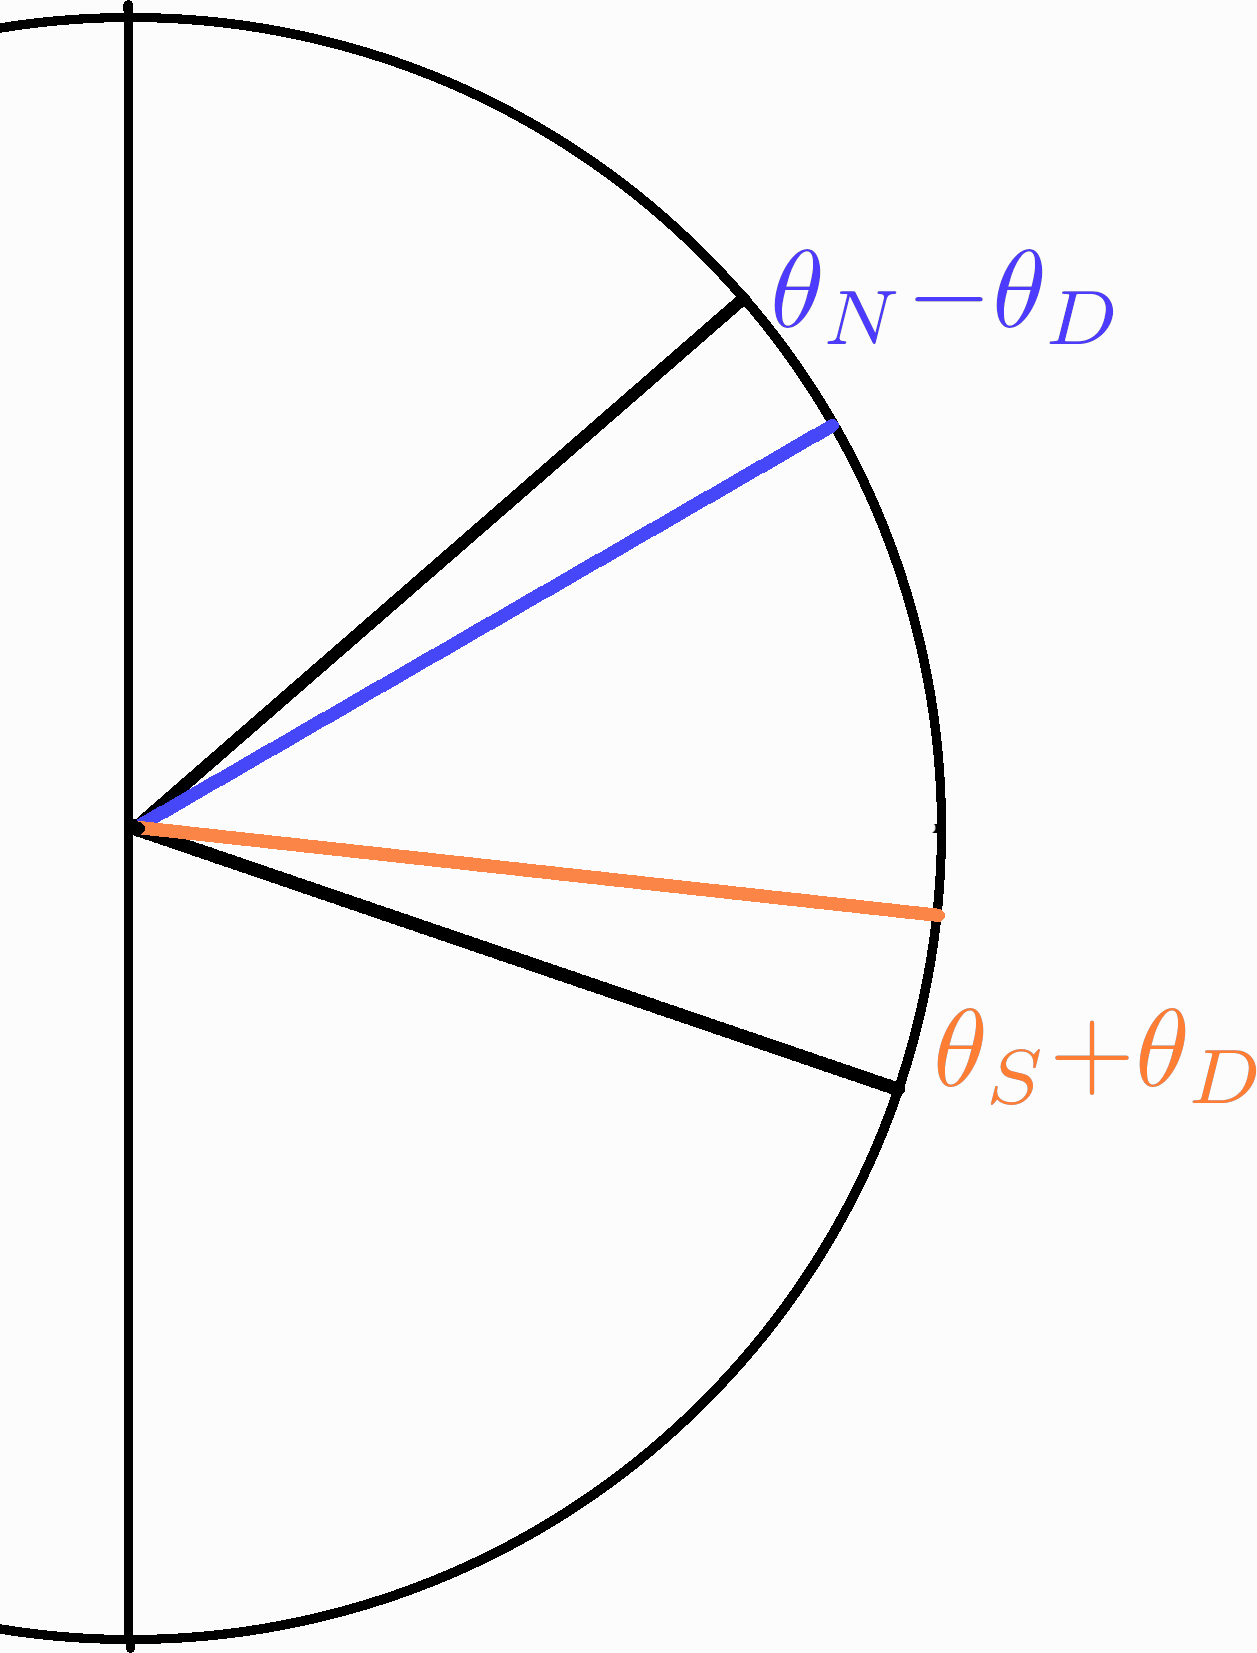
\includegraphics[width=.5\textwidth]{figs/reock_sph_schema.png}
  	\definecolor{ffwwqq}{rgb}{1,0.4,0}
\definecolor{qqttcc}{rgb}{0,0.2,0.8}
\begin{tikzpicture}[scale=.7,line cap=round,line join=round,>=triangle 45,x=1cm,y=1cm]
\clip(-3.059616031054939,-5.482081270032577) rectangle (9.99814205103663,6.011797314398574);
\draw [shift={(1.39,0.41)},line width=2.5pt]  plot[domain=-1.6009682543555996:1.540624399234193,variable=\t]({1*4.972263066250617*cos(\t r)+0*4.972263066250617*sin(\t r)},{0*4.972263066250617*cos(\t r)+1*4.972263066250617*sin(\t r)});
\draw [line width=2.5pt] (1.54,5.38)-- (5.827220035894456,2.6537643265407334);
\draw [line width=2.5pt,dashed,color=qqttcc] (1.54,5.38)-- (6.248241510524688,1.468720655043056);
\draw [line width=2.5pt,dashed,color=ffwwqq] (1.54,5.38)-- (4.287651725431555,-3.63067005311044);
\draw [line width=2.5pt] (1.54,5.38)-- (3.2041318882884013,-4.219505966287888);
\draw [shift={(-3.44,-0.94)},line width=2.5pt,color=qqttcc]  plot[domain=0.23697883378697754:0.3678716704111534,variable=\t]({1*10.308093907216794*cos(\t r)+0*10.308093907216794*sin(\t r)},{0*10.308093907216794*cos(\t r)+1*10.308093907216794*sin(\t r)});
\draw [shift={(-1.36,5)},line width=2.5pt,color=ffwwqq]  plot[domain=5.174361549076037:5.291583521566141,variable=\t]({1*10.679475642558485*cos(\t r)+0*10.679475642558485*sin(\t r)},{0*10.679475642558485*cos(\t r)+1*10.679475642558485*sin(\t r)});
\draw [shift={(1.14,0.48)},line width=2.5pt]  plot[domain=-1.146403466819911:0.41822432957922906,variable=\t]({1*5.925672957563554*cos(\t r)+0*5.925672957563554*sin(\t r)},{0*5.925672957563554*cos(\t r)+1*5.925672957563554*sin(\t r)});
\draw (5.491369061245417,3.7324761595710585) node[anchor=north west] {\color{qqttcc}\LARGE$\kappa_N$};
\draw (2.165325805609785,-4.401351535876993) node[anchor=north west] {\color{ffwwqq}\LARGE$\kappa_S$};
\draw (6.886529002546884,-0.7488678952988525) node[anchor=north west] {\LARGE$\kappa$};
\end{tikzpicture}
  	\caption{The points along the line of longitude which define the three caps of interest.  $\kappa_N$ and $\kappa_S$ are the same size and defined by angles of the same measure.}
  	\label{fig:reock_sphere_schema}
  \end{figure}
  
  We define the region $\kappa_N'$ as $\kappa\ssm\kappa_N$ and $\kappa_S'$ as $\kappa\ssm\kappa_S$.  That is, each of these is formed by deleting the corresponding smaller cap from $\kappa$.  Since $\kappa_N$ and $\kappa_S$ have the same area and the smallest bounding cap of 
  $\kappa_N'$ and $\kappa_S'$ is just $\kappa$ itself, these two regions have identical Reock scores on the sphere.  
  Indeed, one can observe that $\kappa_N'$ is the 
  $180$ degree rotation of $\kappa_S'$ about the center of $\kappa$.
  
  However, under the stereographic projection, these regions no longer have the same Reock score in the plane.  The stereographic projection will send our half-great circle to a ray in the plane emanating from the origin and all spherical caps to planar circles, so the stereographic projection will send our spherical regions $\kappa_N'$ and $\kappa_S'$ to planar regions $\varphi(\kappa_N')$ and $\varphi(\kappa_S')$ which can be constructed from circles with their centers along this ray.
  
  The stereographic projection sends the point on the sphere on our half-great circle corresponding to angle $\theta$ to the point in the plane at distance $2\tan(\theta)$ from the origin along our ray.  Thus, $\varphi(\kappa)$ is a circle with diameter $2\tan(\theta_N)-2\tan(\theta_S)$, $\varphi(\kappa_S)$ has diameter $2\tan(\theta_S+\theta_D)-2\tan(\theta_S)$ and $\varphi(\kappa_N)$ has diameter $2\tan(\theta_N)-2\tan(\theta_N-\theta_D)$.  Similarly to their construction on the sphere, $\varphi(\kappa_N')$ and $\varphi(\kappa_S')$ are equal to $\varphi(\kappa)\ssm \varphi(\kappa_N)$ and $\varphi(\kappa)\ssm \varphi(\kappa_S)$, respectively.  We can further observe that $\varphi(\kappa)$ is the smallest bounding circle of both regions in the plane.
  
  However, these two regions do not have identical Reock score in the plane, since $\varphi(\kappa_S')$ has a larger area (and therefore strictly better Reock score) than $\varphi(\kappa_N')$.  To see this, we will show that the area of $\varphi(\kappa_N)$ is strictly \textit{greater} than that of $\varphi(\kappa_S)$. Since all of these regions are circles, it suffices to show that the diameter of $\varphi(\kappa_N)$ is strictly {greater} than that of $\varphi(\kappa_S)$.  We can write
  
  \begin{align*}
  \mathrm{diam}_{\varphi(\kappa_N)} - \mathrm{diam}_{\varphi(\kappa_S)} &= \left(2\tan(\theta_N) - 2\tan(\theta_N-\theta_D)\right) - \left( 2\tan(\theta_S+\theta_D) - 2\tan(\theta_S) \right)\\
  &= \left(\tan(\theta_N) - \tan(\theta_N-\theta_D)\right) - \left( \tan(\theta_S+\theta_D) - \tan(\theta_S) \right),
  \end{align*}
  
and the claim follows by showing that this quantity is greater than zero.  We then write 

$$0< \left(\tan(\theta_N) - \tan(\theta_N-\theta_D)\right) - \left( \tan(\theta_S+\theta_D) - \tan(\theta_S) \right),$$
 or equivalently,
 $$\tan(\theta_N) + \tan(\theta_S) >   \tan(\theta_N-\theta_D) + \tan(\theta_S+\theta_D). $$

This inequality follows from the fact that $\tan(\theta)$ is convex on the relevant interval,\footnote{Equivalently, since the derivative of $\tan(\theta)$ exists on this interval, we can observe that the second derivative of $\tan(\theta)$ is always positive between $0$ and $\pi$, so it is convex.} $0<\theta<\tfrac{\pi}{2}$.

Since  the diameter of $\varphi(\kappa_N)$ is strictly {greater} than that of $\varphi(\kappa_S)$, we have the same relation on their areas.  This implies that the area of $\varphi(\kappa_N')$ is smaller than that of $\varphi(\kappa_S')$, and therefore has a worse Reock score in the plane. 
   
  
\end{proof}


\begin{figure}[h]
	\centering
	%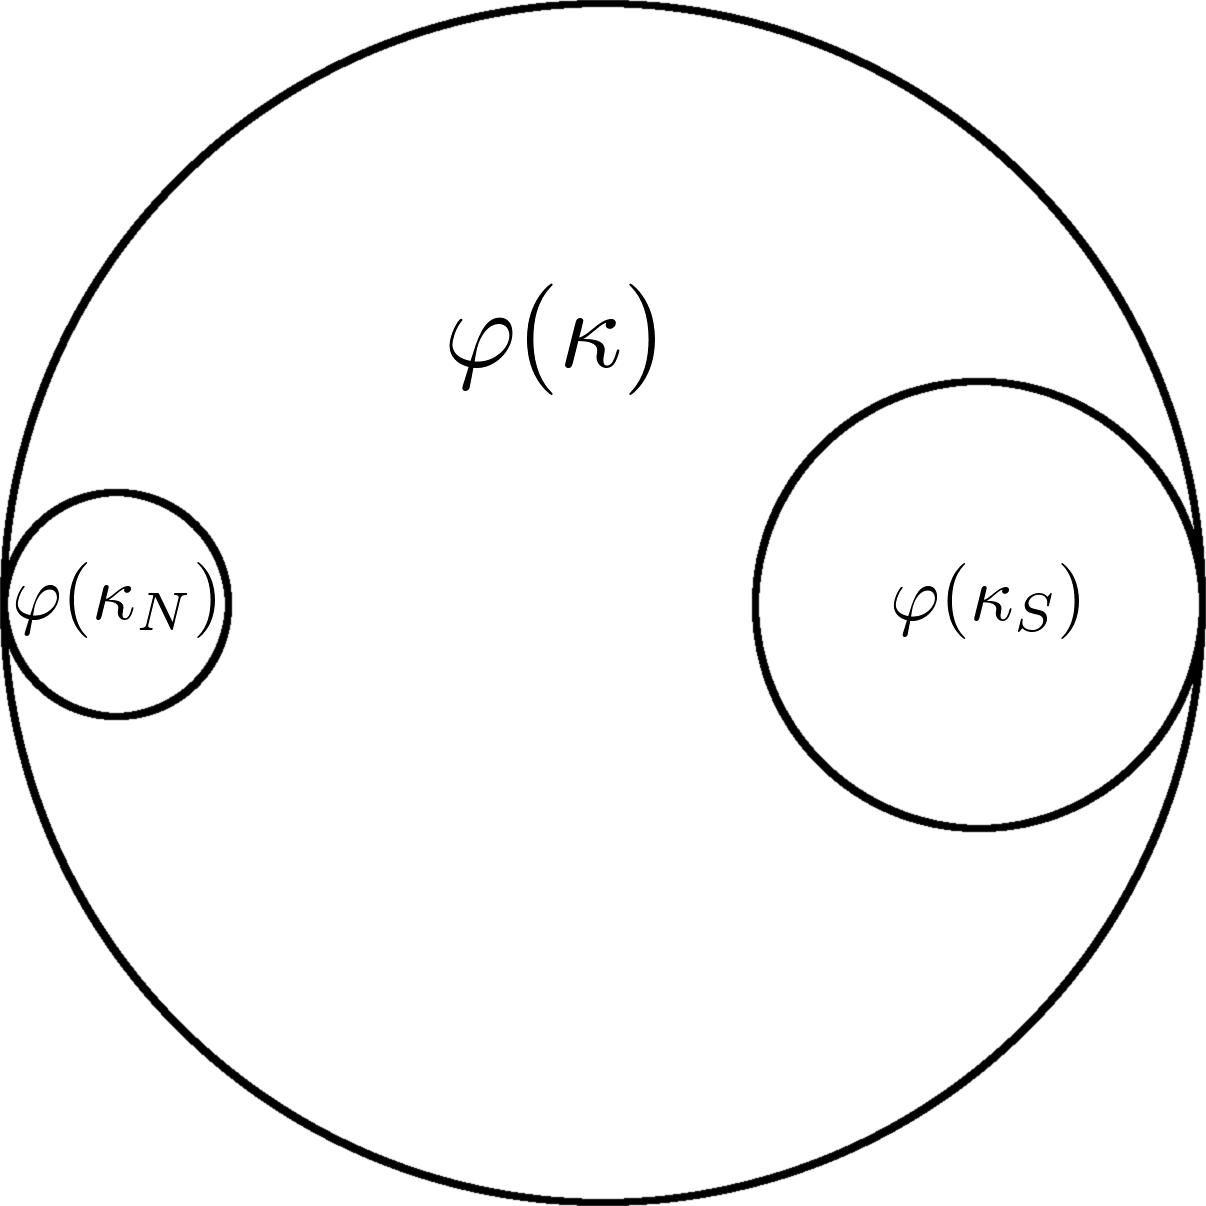
\includegraphics[width=.3\textwidth]{figs/differentkappa.png}
	\definecolor{ffwwqq}{rgb}{1,0.4,0}
\definecolor{qqttcc}{rgb}{0,0.2,0.8}
\definecolor{ffffff}{rgb}{1,1,1}
\begin{tikzpicture}[line cap=round,line join=round,>=triangle 45,x=1cm,y=1cm]
\clip(-1.5345900416212293,-1.8378020210755637) rectangle (12.352141276249895,5.634581973778897);
\draw [line width=3.6pt,color=ffffff,domain=-1.5345900416212293:12.352141276249895] plot(\x,{(--12-0*\x)/6});
\draw [line width=3.6pt,color=ffffff] (5,-1.8378020210755637) -- (5,5.634581973778897);
\draw [line width=2pt] (5,2) circle (3cm);
\draw [line width=2pt,color=ffwwqq] (5,4.333487609592256) circle (0.6665123904077443cm);
\draw [line width=2pt,color=qqttcc] (5,0.5064329039354236) circle (1.5064329039354236cm);
\draw [color=ffwwqq](4.231779936433449,3.726140770933494) node[anchor=north west] {\LARGE$\varphi(\kappa_S)$};
\draw [color=qqttcc](4.231779936433449,0.840353304513867) node[anchor=north west] {\LARGE$\varphi(\kappa_N)$};
\draw (4.331779936433449,2.8655016217034057) node[anchor=north west] {\LARGE$\varphi(\kappa)$};
\end{tikzpicture}
	\caption{The images in the plane of the three caps $\kappa$, $\kappa_N$, and $\kappa_S$.}
	\label{fig:reock_schema}
\end{figure}

Piecing this together yields:
\begin{theorem}
  There is no map projetion from the sphere to the plane which preserves the ordering of Reock scores.
\end{theorem}

\begin{proof}
	  Since such a projection must send caps on the sphere to circles in the
	plane, it must be the composition of the stereographic projection with
	a scaled isometry of the plane.  Since scaled isometries preserve
	Reock scores and therefore their ordering, a Reock score
	order-preserving projection from the sphere to the plane cannot exist
	if the stereographic projection does not preserve the ordering.  By
	the constructed counterexample, it does not, and therefore there is no
	such Reock score ordering map projection.
\end{proof}
